%Your reference code for the next loading is:
%Note! There is a percentage sign at the beginning of the line!

%H8KLCAAyEsKVYQIDw5VYTW/DmkAQw70rET02wqzDpmNnPyrDtcKSKjnCtcKXXkMOTnAawqsuIMKCwprCpBHDv8K9Y8OAwoDCi3BIAsOpZsKNwoTCmV3Dr3vDs3ZmZ3HDp8O8wrHDl8KZPMKMw7Jew6dTwq9zWsKWw4XDqFbDr8KPe8KdwqvDoWDCkg8masOXEcK3wpPDscOww6d8w4zCh8KTwrPDqsKawo3CuS7DinJuPMKNwqdfTsOnw4bCshjDpHdFf3LCoz1gw6zDgsOSw49uK8ODw7nChcO+w64Xwr/DssOBbTEcw5TCk2fDowXDjn3DtcKMwo54w5DDry7DglRvw7NBf8OVwod1J0zCtR0nw4cdw5vDiFPDosOkV8O0wrYywqdEwqlTwpvDrsKSOntpY8K/w6xzwonCh01Fw7Bfw7LDncOQwqLDvcO3w7xqwpINfsKUT8OwD1Bdw79rwr8xKMKefRQgwrDDqMKpThHCg0ASfMKIwoHCo8OeWcKbwqp3L8OdwpHDnsOBw6LDkMO7wo4tScKfw746w4XDp8OsS8KpwqnDv8Ocwp3DqSTDv1PDpMOjdsOyZ2fCoMOtDUpaw4spwqgKwqvCqjcbwo/Ch3czBsOdGcO2RMKrw4J8w7hNwp7DtWcdZTbDicOvw6fCnVlRwq7Cm8KmCy/Dh8ODcsOxw5AIwrdXw5YRbcOpS1FDw5zCpcKwHlxCNCTDm0VMXcODHU/ChcKHwpXCsEbDmsKUD8OfSxpTSwV4woM8ZmnDsFjCl3BJQ8KSVHDDt8OTw7FhFVzDsWDDmcOYCcKlwqUawqbClMOFT8KXw4LDg8KKw5jCtcOSZMKywq7DosKKSMKXJMONPzsNwq3CtsOmM0rCsmfCosKXO8KQQhg/woPDvcKBw6N4SSRsbAZdwpQWGcOTesOjUDHDnMKow6vDrh3CnMOtX8OhQVJFbQfDugc+wp3CijTCqTTDqsOawpLCicOdw5zCkMK/fsOLKsO/w5tkBFjDijjCq0IGGMKiCMKgWj04YnHCi8O5WQzCocOYCBZsIER/wrzDpMKvEynCpVfCg8KTNUgMwoQcFcOHE3MNDUYiecO9woDCoMKQY2pgw7MewrBRDMOEw6DCgwdkEg8cw6oFDsOGecKlE8Kjw5dmw4lJA1vDtsKAw50VZ8KCIMKGGDDCqMKwwq5+wolFBsOEEXjDpkgxRGrCuh3DtgHDjcOOwrBjw4/DqnpAw6fCgsKvQw3DkcKICxbDiDokAXYNbMOcwovDpsOMRsKDw5sHw7TClgXDgMOVwprCu2BidMOKw4crN8OnbRPCm8OwJcOYa8O7w4UMw5vCksORKMKzTizCicKLEcOqMMOHwojCmgPDnjFrw7TDj1bCpAHCnsOtAcKbwpwzTifCty4iWyHCu8KAw7ZgSMKDH8KcMFHCkGDDt8KOw5wlZ8KswobCmELDuBB9XMK+LsOFw4gmRMOrwr3DphnCgMOFBsOyw6U+fCbCo8OucsKwFMKtFcKGZXpJwqzCkl5IV8KaRDg2wpB7w5rCrsOHw5nDlWPDtsOxcsO6wphNwo8+H8KtTMOTw4fDi8Oaw7A7G8KPbsKKworDpkXDpy/ChMKbwqpIMRsAAA==

%Your TikZ code is as follows:
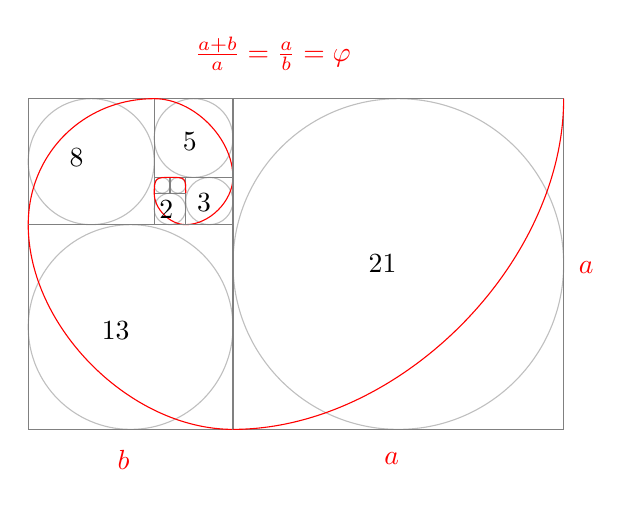
\begin{tikzpicture}
	\draw[draw=lightgray, thin, solid] (0.10,0.10) ellipse (0.10 and 0.10);
	\draw[draw=lightgray, thin, solid] (0.30,0.10) ellipse (0.10 and 0.10);
	\draw[draw=lightgray, thin, solid] (0.20,-0.20) ellipse (0.20 and 0.20);
	\draw[draw=lightgray, thin, solid] (0.70,-0.10) ellipse (0.30 and 0.30);
	\draw[draw=lightgray, thin, solid] (0.50,0.70) ellipse (-0.50 and -0.50);
	\draw[draw=lightgray, thin, solid] (-0.80,0.40) ellipse (-0.80 and 0.80);
	\draw[draw=gray, thin, solid] (0.00,0.20) rectangle (0.20,-0.00);
	\draw[draw=gray, thin, solid] (0.20,0.20) rectangle (0.40,0.00);
	\draw[draw=gray, thin, solid] (0.00,0.20) rectangle (0.40,-0.40);
	\draw[draw=gray, thin, solid] (0.00,0.20) rectangle (1.00,-0.40);
	\draw[draw=gray, thin, solid] (1.00,-0.40) rectangle (0.00,1.20);
	\draw[draw=gray, thin, solid] (0.00,1.20) rectangle (-1.60,-0.40);
	\draw[draw=red, thin, solid] (0.40,0.00) .. controls (0.40, 0.20) and (0.40, 0.20) .. (0.20,0.20);
	\draw[draw=red, thin, solid] (0.20,0.20) .. controls (0.03, 0.20) and (0.00, 0.20) .. (0.00,0.00);
	\draw[draw=red, thin, solid] (0.00,0.00) .. controls (0.00, -0.20) and (0.20, -0.40) .. (0.40,-0.40);
	\draw[draw=red, thin, solid] (0.40,-0.40) .. controls (0.70, -0.40) and (1.00, -0.10) .. (1.00,0.20);
	\draw[draw=red, thin, solid] (1.00,0.20) .. controls (1.00, 0.70) and (0.50, 1.20) .. (0.00,1.20);
	\draw[draw=red, thin, solid] (0.00,1.20) .. controls (-0.90, 1.20) and (-1.60, 0.50) .. (-1.60,-0.40);
	\draw[draw=lightgray, thin, solid] (-0.30,-1.70) ellipse (1.30 and 1.30);
	\draw[draw=gray, thin, solid] (-1.60,-0.40) rectangle (1.00,-3.00);
	\draw[draw=red, thin, solid] (-1.60,-0.40) .. controls (-1.60, -1.70) and (-0.30, -3.00) .. (1.00,-3.00);
	\draw[draw=lightgray, thin, solid] (3.10,-0.90) ellipse (2.10 and -2.10);
	\draw[draw=gray, thin, solid] (1.00,-3.00) rectangle (5.20,1.20);
	\draw[draw=red, thin, solid] (1.00,-3.00) .. controls (3.10, -3.00) and (5.20, -0.90) .. (5.20,1.20);
	\node[black, anchor=south west] at (-0.06,-0.45) {$2$};
	\node[black, anchor=south west] at (0.42,-0.36) {$3$};
	\node[black, anchor=south west] at (0.24,0.42) {$5$};
	\node[black, anchor=south west] at (-1.20,0.21) {$8$};
	\node[black, anchor=south west] at (-0.79,-1.98) {$13$};
	\node[black, anchor=south west] at (2.60,-1.13) {$21$};
	\node[red, anchor=south west] at (2.80,-3.57) {$a$};
	\node[red, anchor=south west] at (5.27,-1.15) {$a$};
	\node[red, anchor=south west] at (-0.59,-3.63) {$b$};
	\node[red, anchor=south west] at (0.39,1.43) {$\frac{a+b}{a} = \frac{a}{b} = \varphi$};
\end{tikzpicture}

%File was created at 2021. 11. 17. 15:31:14